\documentclass[a4paper, 11pt, lualatex, ja=standard, twocolumn]{bxjsarticle}

\usepackage{graphicx} % 画像
\usepackage{tabularx} % 表

\usepackage{amsmath}  % 数式
\usepackage{url}      % URL
\usepackage{siunitx}  % SI単位

% フォント設定
\usepackage[no-math, deluxe, bold, haranoaji]{luatexja-preset}

\usepackage{layout}   % レイアウト確認

\renewcommand{\tablename}{Table}    % 表番号フォーマットをTableへ
\renewcommand{\figurename}{Fig.}    % 図番号フォーマットをFig.へ

\renewcommand{\baselinestretch}{0.8}    % 行間の調整

% レイアウトパラメータを変えなきゃならないときこれを使う
%\geometry{left=25mm,right=25mm,top=25mm,bottom=25mm, includefoot}

\title{\Huge タイトル}
\author{\huge 書いた人の名前}
\date{\today}

\begin{document}
  \maketitle

  \section{Hello, Lua\LaTeX !!!}
    Lua\LaTeX デビュー!!

  \section{二段組み}
    Lua\LaTeX でも普通に二段組みの文書が作れました.
    卒業論文などに使いましょう.
  
  \section{図の貼り方}
    図の貼り方はup\LaTeX の時と同じです.
    figure環境を使うことで画像を貼ることが出来ます.
    PDF画像の他,JPEGやPNGもそのまま貼ることが出来ます.
    但しEPS画像はおすすめしません.時代遅れです.

    \begin{figure}[h]
      \centering
      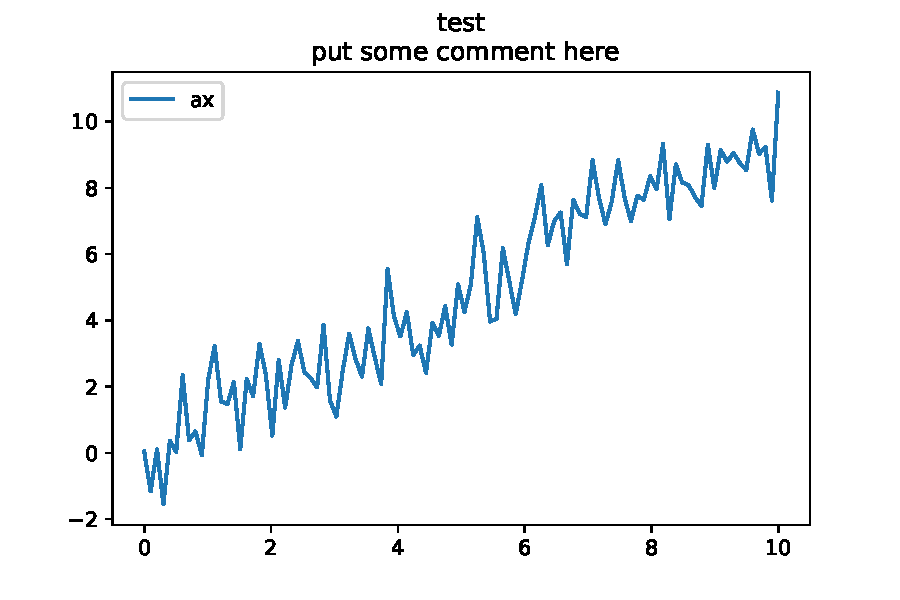
\includegraphics[width=60truemm, clip]{images/graph_sample.pdf}
      \caption{Sample Picture}
      \label{fig:sample}
    \end{figure}
  
  \section{数式の描き方}
    普通に\LaTeX の書き方で書けます.
    \begin{equation}
    {}^0\!T_{1}=\begin{pmatrix} C_{1} & -S_{1} & 0 & 0 \\ S_{1} & C_1 & 0 & 0 \\ 0 & 0 & 1 & 0 \\ 0 & 0 & 0 & 1 \end{pmatrix}
    \end{equation}

\end{document}